Data streams are crucial in  the modern connected Internet 
world, and they have attracted the attention of researchers worldwide. Given the important
applications of data streams--such as IoT, social networks, and surveillance--mining them is becoming a more and more important topic to explore. 
However, data stream mining is also a challenging task due to its distinctive nature. 
For example, a data stream is theoretically infinite in length, therefore, its volume
is very large. Meanwhile, it is possible that with high velocity of data arrivals, class labels are not available immediately after the arrival of new data instances, which is hard to update the model. 
These properties have distinguished data 
stream mining significantly from traditional data mining problems \cite{haque2016SAND}.


% This paragraph talks about stream classification
Classification techniques solve problems of identifying which of a certain set of categories
that a new instance belongs. Normally it is assumed that the classification model, which is
trained by source data with true labels, is also representative to target data.
However, this assumption does not always hold in real world applications. Since data streams are generated
by non-stationary processes, it is possible that arbitrary changes may be introduced to data streams during generation. 
Due to this shift in concept, using a model trained by old source data may introduce bias
in prediction \cite{herlihy1993methodology}.
In this case, a classification model trained by previous data is no longer representative to test
data in the future, and will perform poorly in prediction due to bias. Thus, the model needs proper updates to adapt the current concept.
When it comes to the setting of multiple streams, this problem becomes even
more challenging. The problem setting is described and motivated by a MultiStream
Classification (MSC) algorithm \cite{chandra2016adaptive}. Two data streams are
involved simultaneously under this setting. One is referred as the source stream,
which contains data instances with class labels generated from a non-stationary
process. The other is referred as the target stream, which consists of data generated
from another non-stationary process. Since getting true labels for target streams needs tremendous validation by human experts, here
we assume that true labels of target stream will not be available after the prediction.  

% This paragraph talks about domain adaptation
We consider a domain adaptation setting within the multistream classification framework. There is a need to address machine learning tasks of building 
models in a one domain by using information available from another related domain. In
this case, knowledge from the source domain (stream) can be transferred to the target domain (stream) to
help get high prediction accuracy. This transfer process is important in many 
circumstances where labels in a certain domain are limited or too expensive to obtain \cite{arnold2007comparative, hoi2014libol}, which fits the need of multistream by nature.
% For example, it is difficult to collect labeled sensor
% data from personal devices, while rich information from social media messages are available, such as 
% activities and locations. Thus, knowledge from social media can be transferred to
% the physical world to address the ubiquitous computing tasks \cite{wei2016instilling}. 

In practice, most existing approaches usually process the streams in batches. Also, it is normally 
assumed that training data are provided as a whole in advance \cite{pan2010survey}. However, such assumptions
do not always hold in real world applications, since under a data stream setting 
all instances may arrive in a sequential manner. Take online spam email detection for example \cite{chen2015opinion}. 
Normally, a classifier is built by using a static training dataset, and it is trained in batches to
detect spam emails as accurately as possible. However, the very definition of spam varies from 
person to person. In this case, the transfer of knowledge to personalize the spam detector for each 
individual becomes critical. Even for a specific person, the definition of spam could change over time. During a certain
time period one may consider an advertisement from Zillow to be spam. When he starts to consider buying a house,
Zillow ads are not spam for him anymore. Such problem can be formulated as a multistream learning task, the 
objective of which is to build an online prediction model for the target domain by using information 
available in the source domain with distinct feature space. Compared to the previous example, this task 
is more challenging, as the concept is evolving in the data streams simultaneously in heterogeneous source and target streams.

\begin{figure}[t]
\centering
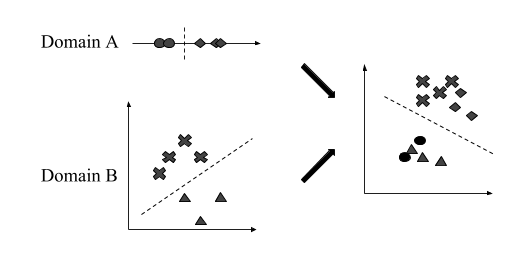
\includegraphics[width=0.8\columnwidth]{Figures/feature_projection.png}
\caption{Feature Space Projection}
\label{fig:featureprojection}
\end{figure}

To sum up, the problem that we are trying to solve involves the multistream setting for different domains with differing feature space dimensions. 
More specifically, two data streams have heterogeneous feature spaces, and this is the aspect which no researchers have been working on in the past. 
Meanwhile, features across two domains may not correspondent to each other. Still, as stated above, these two stream should be related so that domain adaptation will make sense. 
For example, to setting up a monitoring system of global pollution level, different countries may monitor different sets of parameters: some of them may overlapping, some of them may be special to use in certain countries. 
In the end, we want to classify the pollution level for all the countries by the same category. Under this circumstance, how to properly adapt domains becomes critical.

% \textcolor{red}{My Hint: Here I need to emphasis that: 1. source and target streams have different dimension of features. 2. features does not have any correspondence. 3 two datasets are related.}

This paper proposes a framework, called MultiStream Domain Adaptation (MSDA), to handle the issues described above. The
main idea is to find a common feature space for two distinct data streams. This idea is demonstrated in Figure ~\ref{fig:featureprojection}. In this case, data in domain A are one-dimensional and in domain B are two-dimensional. By applying the proposed projection algorithm, we
try to find a latent feature space that the distributions in original and latent feature space are similar. 
Meanwhile, the structure of data should be preserved, which means distinct classes are still far
apart, and the decision boundaries for different categories should still be preserved.
Thus the core problem here is to find a feature space that maximize the similarity between
original and projected latent feature space. Main contributions of this paper are as follows:

\begin{enumerate}
\item A new data stream classification setting with two independent non-stationary streams is created. Features in two streams are not identical. Class labels in the target stream are predicted by data instances from the source stream.
\item An embedding-based domain adaptation method is introduced to address the challenges of adapting source and target domains in a non-stationary environment.
\item A concept drift detection method is deployed under the new multistream setting with domain adaptation. Under this setting, true labels in the target stream is not required, while only true labels in the source stream is used. 
\item Our approach is empirically evaluated over several benchmark datasets, and the results are compared with baseline methods. The performance of our proposed method is significantly better than the other three methods.
\end{enumerate}

The rest of the paper is organized in the following ways. Section~\ref{sec:relatedwork} discusses related work; Section~\ref{sec:problemformulation} provides the mathematical formulation of the problem that we solve; Section~\ref{sec:proposedapproach} describes the details of our proposed solutions; Section~\ref{sec:experinment} illustrates our experimental results; and finally, Section~\ref{sec:conclusions} concludes our paper and offers directions for further work.

